%!TEX root = ../dissertation.tex
\begin{savequote}[75mm]
``We can change our tools and then our tools change us"
\qauthor{Jeff Bezos - Entrepreneur}
\end{savequote}

\chapter{A11Y Tool}
With the successful completion of the A11Y Guide sufficient knowledge had
been gained within the accessibility domain to enable the production of a
tool to identify issues. The fundamental idea behind the tool is to reduce
the feedback loop (and thus the price) of discovering accessibility issues. To
keep the project to a sensible scope the tool will form the "means" by which
accessibility testing could be undertaken but will be limited in the number
of accessibility issues it will identify.

\section{Preparation}
\subsection{Current Process}
As mentioned by John in section \ref{quote:john} accessibility is often
unfortunately an item which is ``Left until later" or ``Poorly tested" early
on in the project. Fig.~\ref{fig:process_1_} and Fig.~\ref{fig:process_2}
demonstrate two slightly different methods projects go down. The common
problem is that issues are only detected late in the development lifecycle.
The problems that are found tend to be similar and remdiation is often a
painfully repetitive process.

\subsection{Current solutions}
\label{sec:currentSolutions}
With this in mind a survey of the current landscape of accessiblity tools was
undertaken. Fortunately when producing the A11Y guide a list of current
testing tools had been collated which made this step relatively easy.

Of the tools each plugs into different possible points throughout the
development phase:
 \begin{itemize}
 \item The IDE - Most modern IDE's have a means for plugging in linting tools
  to check structure.
 \item The CLI - Rulset libraries such as ESLint and HTMLLint can execute
 against your code and report issues to the console. They can even be part of
  a wider continuous integration setup
  \item The Browser - By bootstrapping through a `Bookmarklet' this method
  highlights issues in a browser window, often producing a report.
 \end{itemize}

Performing more research into how the IDE tools work they are typically just
wrappers around. The table below shows the good/bad points surrounding each tool

\begin{table}[h!]
\centering
\begin{tabular}{ |c|c|c| }
 \hline
 \thead{Tool} & \thead{Good} & \thead{Bad}  \\
 \hline
 \hline
 Axe  & \makecell{No false positives \\
  Very configurable \\
   Multiple languages}& \makecell{By avoiding false positives it limits the
   tests\\
   Lots of manual setup required} \\
 \hline
 \makecell{HTML Code \\ Sniffer} & \makecell{Very visual \\ Configurable level
 error or
 warning \\ Can go straight to problem element}&
 \makecell{Cant target a specific WCAG level \\ Not very configurable \\
 Bookmarklets are becoming legacy} \\
 \hline
  Tota11y & \makecell{Helps teach accessibility \\ Can assess page structure
  } & \makecell{Not very comprehensive \\ Bookmarklet} \\
 \hline
 \makecell{ESLint JSX \\ A11Y (IDE)} & \makecell{Fast feedback \\ Plugs into
 current tooling } &
 \makecell{Can only detect minor issues \\ } \\
 \hline
\end{tabular}
\end{table}

\subsection{Requirements}
\label{ref:requirements}
Similar to the A11Y Guide requirements were defined following Dan North's
``Whats in a story" model.

\begin{center}
 \begin{tabular}{| c |}
 \hline
 As a developer \\
 \hline
 I want to be able to customise the ruleset \\
 So that my projects accessibility requirements can be assessed \\
 \hline
 I want to be able to run the tool through multiple methods \\
 So that I can run it locally and as part of a wider Continuous integration \\
 process \\
 \hline
 I want to be able to have errors categorised \\
 So that I can prioritise which ones to fix first \\
 \hline
 I want remdediation advice \\
 So that I know how to fix the error \\
 \hline
 I want remediation advice to have more information \\
 So that I can learn about the mistake made \\
 \hline
 (This Project Scope) \\
 I want 20\% of issues on BBC's terribly accessible page to be identified \\
 So the framework can be proved \\
 \hline
\end{tabular}
\end{center}

\section{Design \& Implementation}
\subsection{Proposed Solution}
Fig.~\ref{fig:tool_current_design} demonstrates roughly how most of
the current tools (Tota11y, EsLint) are designed. They typically have tightly
coupled components for applying rules and displaying results which limits the
way in which developers are able to use the tool.

\begin{figure}[H]
\centering
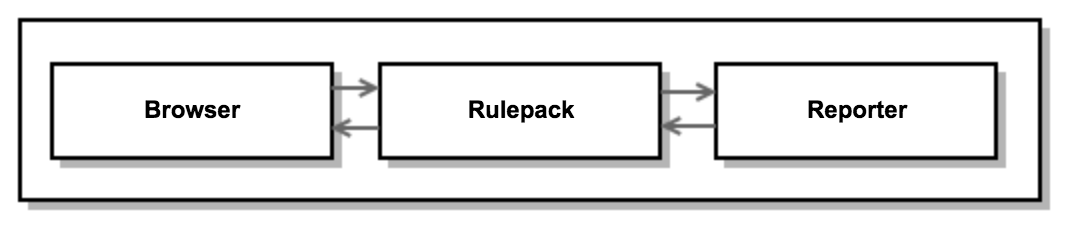
\includegraphics[width=0.8\textwidth]{figures/a11y_tool_current_design}
\captionsetup{justification=centering}
\caption{Current tool design
\label{fig:tool_current_design}}
\end{figure}

With this in mind the design for this tool would focus on reusability and
customisation. Coming from a Java background we tend to apply the inversion
of control principle \citep{DRC} to help decouple the reusable components from
the specific ones. This comes with the added benefit of being able to build
and test specific modules in isolation.
Fig.~\ref{fig:tool_proposed_design} demonstrates the high level design for
how this will be applied to the A11Y Tool. Components shown in grey demonstrate
the possiblites which are opened by using such a design but are out of scope
of this project. The next few sections in the report will document the design
and implementation of each of the components within scope of the project.

\begin{figure}[H]
\centering
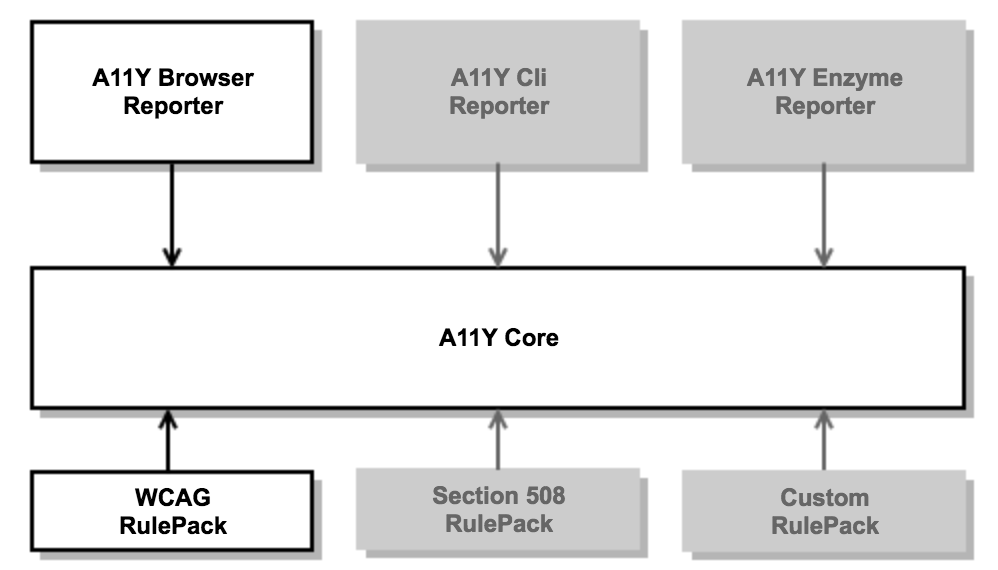
\includegraphics[width=0.7\textwidth]{figures/a11y_tool_proposed_design}
\captionsetup{justification=centering}
\caption{Proposed tool design
\label{fig:tool_proposed_design}}
\end{figure}

\subsection{A11Y Core}
This component offers the fundamental building blocks which enable the
others to function. It defines interfaces and common implementations and
forms a language to use for extensible components. `Checker', `Result' and
`Worker'. These are discussed later in the report.

\subsubsection{Versioning}
Due to other components relying upon A11Y Core's interfaces, versioning of
the api it exposes is important to ensure dependent parties are able to update
efficiently. There are many versioning strategies available and most work on
a form of three digits [major].[minor].[patch]. I always use `Semantic
Versioning' \citep{Semver} due to the clear definition of when each number should
increment.
Patch for bug fixes and non api changes, Minor for API additions which are
backwards compatible and Major when a breaking API change is introduced. Due to this
clarity it is slowly becoming the defacto standard for software development
so is likely to be familiar to others.

\subsubsection{Checker}
A `Checker' offers a method to check content for issues and give detail
about what they are checking for. Fig.~\ref{fig:checker_design} documents the
initial design for `Checker' and its various child implementations.

\begin{figure}[H]
\centering
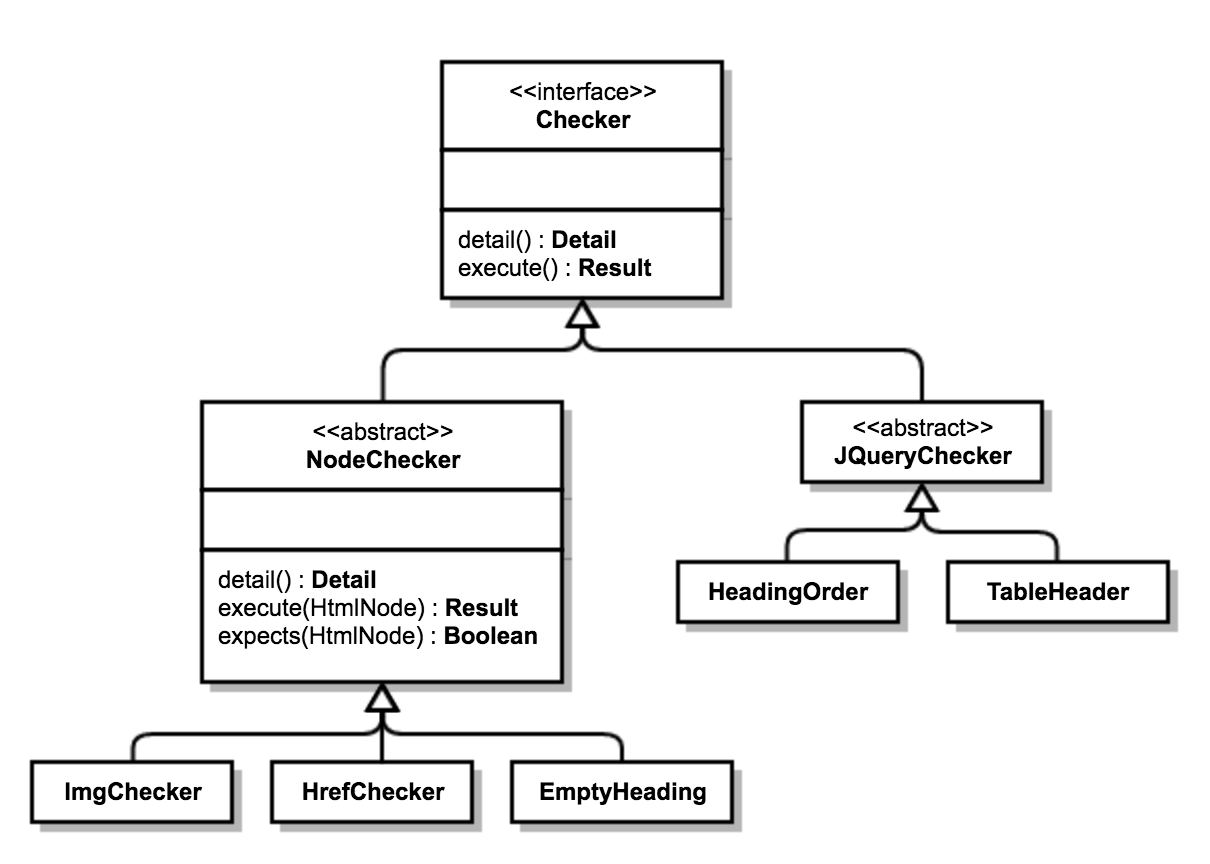
\includegraphics[width=0.6\textwidth]{figures/a11y_tool_checkers}
\captionsetup{justification=centering}
\caption{Proposed `Checker' design
\label{fig:checker_design}}
\end{figure}

Due to EcmaScript's inability to support interfaces I use the constructor to
validate the `instance' for the correct methods at creation time. As these
methods can only exist in child classes it is impossible to create an
instance of `Checker' without them. I felt this was an adequate and efficient
way of creating a framework which others could extend.

\begin{lstlisting}[language=JavaScript]
export default class Checker {
  constructor() {
    this.validateInstance(this.constructor.detail, this.constructor.execute);
  }

  validateInstance(detail, execute) {
    this.validateExists(detail, 'No detail object present');
    this.validateExists(execute, 'No execute method present');
  }

  validateExists(mustExist, error) {
    if(!mustExist) {
      throw new Error(`${this.constructor.name} | ERROR: ` + error);
    }
  }
}
\end{lstlisting}

\subsubsection{Result}
The `Result' class is an outcome of a `Checker'. They hold the node or element
the `checker' checked and the state, Success, Warn, Info or Error.
Error and Warn have an additional property of
remediation which is to be added by the `Checker' to offer a recommended
method to fix the identified issue. This coupling allows for the remediation
to be specific to the exact issue found by the checker. Fig
.~\ref{fig:result_design} demonstrates `Results' inheritance structure. It is
unlikely that anyone would extend `Result' but similar to above it has been
implemented with interfaces.

\begin{figure}[H]
\centering
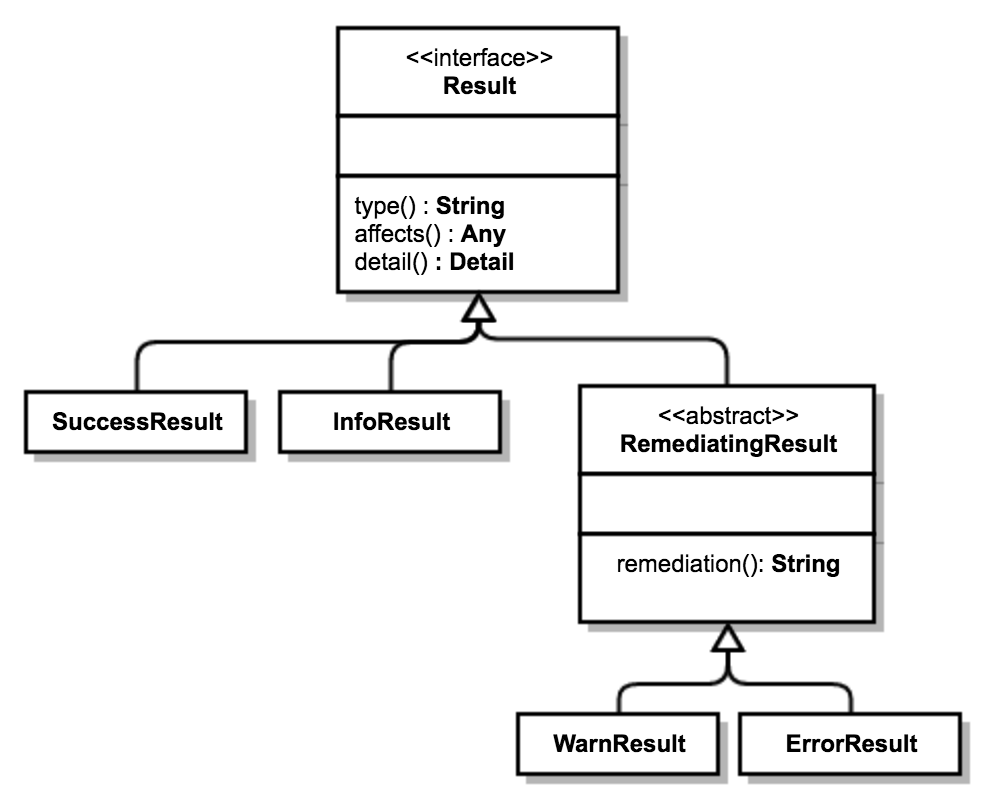
\includegraphics[width=0.6\textwidth]{figures/a11y_tool_result}
\captionsetup{justification=centering}
\caption{Proposed `Result' inheritance structure
\label{fig:result_design}}
\end{figure}

\subsubsection{Worker}
The concept of a `Worker' was added late on during the implementation phase as a
direct result of the performance of `Checker's being poor. Performance issues
were noticeable when iterating around a web pages with a large number of DOM
elements. The worker inverted the for loop and meant that
rather than iterating around the DOM within each `Checker' The DOM was
iterated around only once and each checker was called to perform it's check
only if that DOM node was relevant to it.

`Workers' implement the Singleton Pattern so `Checkers' can be registered from
anywhere. Each individual checker registers itself with it's retrospective
worker. The result of such a design (and the reason this was chosen over others)
is that when a `Checker' is imported into a file it is registered with 'A11Y
Core' and thus available for use. Fig.~\ref{fig:a11y_tool_worker_design}
shows how this works.

\begin{figure}[H]
\centering
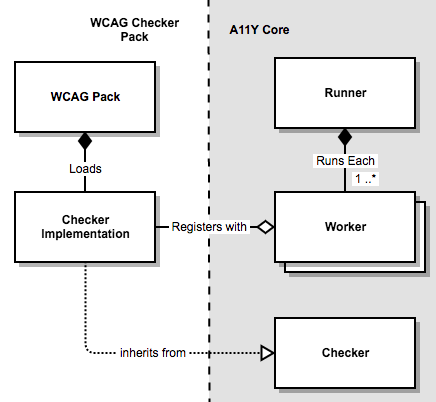
\includegraphics[width=0.5\textwidth]{figures/a11y_tool_worker_design}
\captionsetup{justification=centering}
\caption{Relationships between components and classes
\label{fig:a11y_tool_worker_design}}
\end{figure}

\subsection{A11Y WCAG Checker Pack}
As shown in Fig.~\ref{fig:a11y_tool_worker_design} above `Checker Packs' are
a collection of `Checkers' loaded into a single file. The requirement for a
'Checker Pack' comes from the fact that the accessibility requirements on
projects change. Some might be required to satisfy the WCAG AA others may
require the Section 508 guidelines.

Below is a snippet from the WCAG 'Checker Pack'. Packs are deliberately easy to
create so users of the tool can compose and apply their own rules.

\begin{lstlisting}[language=JavaScript]
import 'checkers/WCAG/HrefChecker.js';
import 'checkers/WCAG/HeadingOrderChecker.js';
import 'checkers/WCAG/TableCaptionChecker.js
\end{lstlisting}

\subsection{A11Y Browser}
The browser component enables the tool to be ran within a web browser. Fig
.~\ref{fig:a11y_tool_browser_design} shows how this fits in with the other
components.

\begin{figure}[H]
\centering
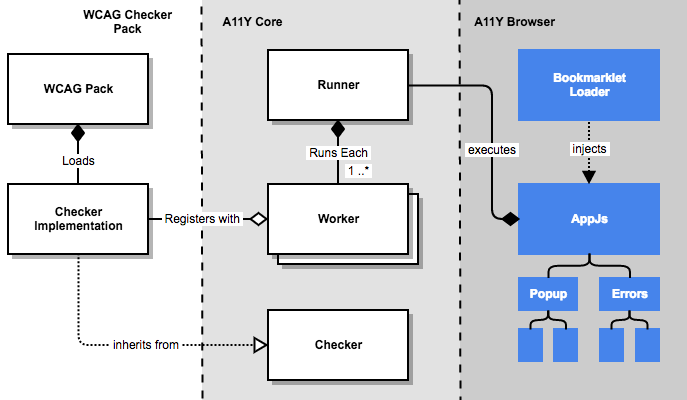
\includegraphics[width=0.75\textwidth]{figures/a11y_tool_browser_design}
\captionsetup{justification=centering}
\caption{How the browser component ties everything together
\label{fig:a11y_tool_browser_design}}
\end{figure}

\subsubsection{Designing the UI}
When surveying the current tools in section \ref{sec:currentSolutions}
the good and bad features were noted and I took some inspiration around
the experience they gave developers. From this and the requirements defined
in section \ref{ref:requirements} a collection of goals which the UI needed
to satisfy were defined:

\begin{itemize}
\item Highlight the html error in place (HTML Code sniffer does this)
\item Categorise errors in error/warning/info (Tota11y does this)
\item Display remdiation (None do this)
\item Have links to the A11Y guide to learn more about the issue
\end{itemize}

HTML CodeSniffer highlights the error with a 'bouncing bubble' as shown in
\ref{fig:codesniffer}. I went for a similar approach shown in
\ref{fig:tool_bubble}.

\begin{figure}[H]
    \centering
    \begin{subfigure}[b]{0.25\textwidth}
        
\includegraphics[width=\textwidth]{figures/codesniffer}
        \captionsetup{justification=centering}
        \caption{HTML Code sniffers bouncing bubble}
        \label{fig:codesniffer}
    \end{subfigure}
    \qquad
    %add desired spacing between images, e. g. ~, \quad, \qquad, \hfill
      %(or a blank line to force the subfigure onto a new line)
    \begin{subfigure}[b]{0.4\textwidth}
        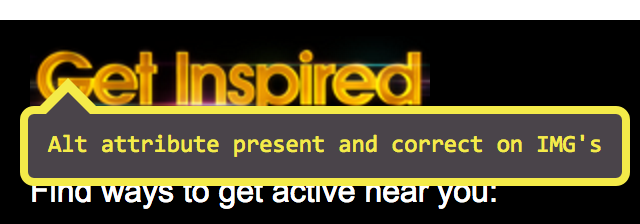
\includegraphics[width=\textwidth]{figures/tool_bubble}
        \captionsetup{justification=centering}
        \caption{A11Y Tool bubble}
        \label{fig:tool_bubble}
    \end{subfigure}
\end{figure}

A problem I had with Tota11y and axe core was logically linking the HTML in
error back to the code in my IDE. I knew the HTML with the error but
without the context of its surrounding elements its difficult to tie it back
to the original source especially when using libraries like React and Angular.
Unfortunately most browsers deliberately limit access to devtools from
javascript. I hypothesised that web developers code web apps with the
'devtools' open. To clarify this I put a message on our internal slack.
Asking people to agree/disagree with the statement. 8 'agreed' and 1 'disagreed'.
From this I decided that the best way to give the context would be to print
the html element to the devtools console. when the element is clicked it takes
the developer to the element in the page source. Similarly advice and
remeidation were also posted here as shown in \ref{fig:remediation}

\begin{figure}[H]
\centering
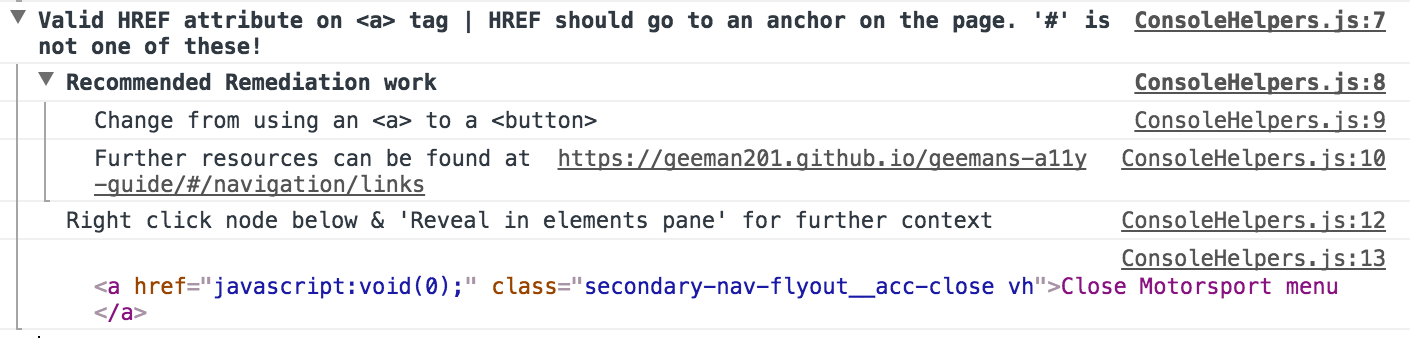
\includegraphics[width=0.75\textwidth]{figures/a11y_tool_remediation}
\captionsetup{justification=centering}
\caption{Console output from A11Y Browser
\label{fig:a11y_tool_remediation}}
\end{figure}

\subsubsection{Bootstrapping the browser}
For the tool to run script tags need to be loaded into the browser. The traditional means is via a
'Bookmarklet' these sit in the bookmark/favourite bar of a users
browser and when clicked execute javascript on the users web page to insert the
 tag and load the tool.

Unfortunately due to Cross Site Scripting issues browsers are implementing
content restrictions whereby the browser blocks scripts from a
domains excluded from a specific meta tag list. When all browsers support
content restrictions the tool would no longer function. An alternate approach
was required and two methods were explored to solve this.

The first a 'browser extension' which would require a small wrapper around
the A11Y Browser tool for each individual browser. This solved the problem.
The tool was loaded into the users browser and worked as expected but a
wrapper would be require packaging for each indivdual browser and there is
talk that vendors are phasing out extensions.

The second, and chosen method, was by allowing the script tag to be inserted
at development time through a script tag. Users could add this to the html
file they wished to test.


%\newthought{Lorem ipsum dolor sit amet},
%
%This chapter should describe what was actually produced: the programs which
%were written, the hardware which was built, the theory which was developed or
%the new scientific knowledge acquired.
%
%For software projects, give a high-level overview of your realisation of the
%design. Describe the general organisation of any body of code, web pages,
%database tables, etc, that you have created. Highlight any particularly
%noteworthy aspects, e.g., specialised algorithms, but avoid excessive low-level
%detail. Diagrams and examples are usually valuable.
%
%For research projects, provide a detailed overview of how the research was
%executed (e.g., participants involved, etc). the research results and their
%analysis. Include a description of any statistical analysis methods used.
%Highlight any particularly noteworthy aspects, e.g., especially interesting
%results. Graphs/charts and examples are usually essential. When reporting
%statistical analysis, do not merely present the statistics without interpreting
%their meaning for the reader – e.g., what are the implications of the findings?
%Where applicable, based on the results and analysis, present a set of
%recommendations, guidelines, or itemised list of contributions to knowledge
%that may be derived from your work.
%
%This section should be answering the question: “What did the project actually
%produce?”
